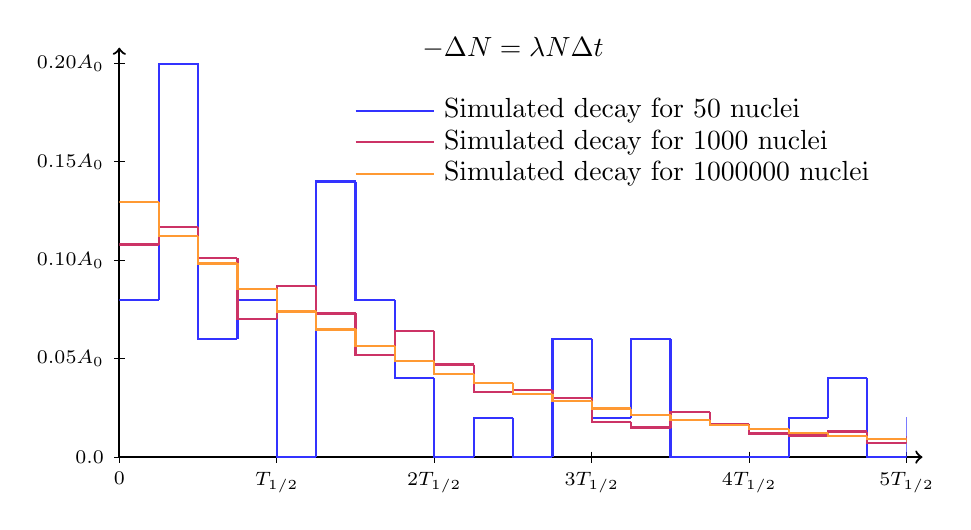
\begin{tikzpicture}
\node[] at (5.0,5.2) {$-\Delta N = \lambda N \Delta t$};
\draw[thick,->] (0.0,0.0) -- (0.0,5.2);
\draw[thick,->] (0.0,0.0) -- (10.2,0.0);
\draw (0,0cm + 2pt) -- (0, 0cm-2pt) node[below] {\scriptsize $0$};
\draw (2,0cm + 2pt) -- (2, 0cm-2pt) node[below] {\scriptsize $T_{1/2}$};
\draw (4,0cm + 2pt) -- (4, 0cm-2pt) node[below] {\scriptsize $2T_{1/2}$};
\draw (6,0cm + 2pt) -- (6, 0cm-2pt) node[below] {\scriptsize $3T_{1/2}$};
\draw (8,0cm + 2pt) -- (8, 0cm-2pt) node[below] {\scriptsize $4T_{1/2}$};
\draw (10,0cm + 2pt) -- (10, 0cm-2pt) node[below] {\scriptsize $5T_{1/2}$};
\draw (0cm+2pt,0.    ) -- (0cm-2pt,0.    ) node[left] {\scriptsize $0.0$};
\draw (0cm+2pt,1.25    ) -- (0cm-2pt,1.25    ) node[left] {\scriptsize $0.05 A_0$};
\draw (0cm+2pt,2.5    ) -- (0cm-2pt,2.5    ) node[left] {\scriptsize $0.10 A_0$};
\draw (0cm+2pt,3.750000093132256    ) -- (0cm-2pt,3.750000093132256    ) node[left] {\scriptsize $0.15 A_0$};
\draw (0cm+2pt,5.    ) -- (0cm-2pt,5.    ) node[left] {\scriptsize $0.20 A_0$};
\begin{scope}[]
\clip (0,0) rectangle (10,5);
\draw[blue!80,thick] (3.0,4.4) -- (4.0,4.4);
\node[right,] at (4.0,4.4) {Simulated decay for 50 nuclei};
\begin{scope}[blue!80,thick]
\draw[] (0.0,1.999999970197678) -- (0.5,1.999999970197678);
\draw (0.5,1.999999970197678) -- (0.5,4.999999925494195) -- (1.0,4.999999925494195);
\draw (1.0,4.999999925494195) -- (1.0,1.4999999776482584) -- (1.5,1.4999999776482584);
\draw (1.5,1.4999999776482584) -- (1.5,1.999999970197678) -- (2.0,1.999999970197678);
\draw (2.0,1.999999970197678) -- (2.0,0.0) -- (2.5,0.0);
\draw (2.5,0.0) -- (2.5,3.4999999478459367) -- (3.0,3.4999999478459367);
\draw (3.0,3.4999999478459367) -- (3.0,1.999999970197678) -- (3.5,1.999999970197678);
\draw (3.5,1.999999970197678) -- (3.5,0.999999985098839) -- (4.0,0.999999985098839);
\draw (4.0,0.999999985098839) -- (4.0,0.0) -- (4.5,0.0);
\draw (4.5,0.0) -- (4.5,0.4999999925494195) -- (5.0,0.4999999925494195);
\draw (5.0,0.4999999925494195) -- (5.0,0.0) -- (5.5,0.0);
\draw (5.5,0.0) -- (5.5,1.4999999776482584) -- (6.0,1.4999999776482584);
\draw (6.0,1.4999999776482584) -- (6.0,0.4999999925494195) -- (6.5,0.4999999925494195);
\draw (6.5,0.4999999925494195) -- (6.5,1.4999999776482584) -- (7.0,1.4999999776482584);
\draw (7.0,1.4999999776482584) -- (7.0,0.0) -- (7.5,0.0);
\draw (7.5,0.0) -- (7.5,0.0) -- (8.0,0.0);
\draw (8.0,0.0) -- (8.0,0.0) -- (8.5,0.0);
\draw (8.5,0.0) -- (8.5,0.4999999925494195) -- (9.0,0.4999999925494195);
\draw (9.0,0.4999999925494195) -- (9.0,0.999999985098839) -- (9.5,0.999999985098839);
\draw (9.5,0.999999985098839) -- (9.5,0.0) -- (10.0,0.0);
\draw (10.0,0.0) -- (10.0,0.4999999925494195) -- (10.5,0.4999999925494195);
\draw (10.5,0.4999999925494195) -- (10.5,0.0) -- (11.0,0.0);
\draw (11.0,0.0) -- (11.0,0.0) -- (11.5,0.0);
\draw (11.5,0.0) -- (11.5,0.0) -- (12.0,0.0);
\draw (12.0,0.0) -- (12.0,0.4999999925494195) -- (12.5,0.4999999925494195);
\end{scope}
\draw[purple!80,thick] (3.0,4.0) -- (4.0,4.0);
\node[right,] at (4.0,4.0) {Simulated decay for 1000 nuclei};
\begin{scope}[purple!80,thick]
\draw[] (0.0,2.699999959766865) -- (0.5,2.699999959766865);
\draw (0.5,2.699999959766865) -- (0.5,2.924999956414104) -- (1.0,2.924999956414104);
\draw (1.0,2.924999956414104) -- (1.0,2.5249999623745687) -- (1.5,2.5249999623745687);
\draw (1.5,2.5249999623745687) -- (1.5,1.7499999739229684) -- (2.0,1.7499999739229684);
\draw (2.0,1.7499999739229684) -- (2.0,2.1749999675899745) -- (2.5,2.1749999675899745);
\draw (2.5,2.1749999675899745) -- (2.5,1.824999972805381) -- (3.0,1.824999972805381);
\draw (3.0,1.824999972805381) -- (3.0,1.2999999806284905) -- (3.5,1.2999999806284905);
\draw (3.5,1.2999999806284905) -- (3.5,1.5999999761581425) -- (4.0,1.5999999761581425);
\draw (4.0,1.5999999761581425) -- (4.0,1.174999982491136) -- (4.5,1.174999982491136);
\draw (4.5,1.174999982491136) -- (4.5,0.8249999877065423) -- (5.0,0.8249999877065423);
\draw (5.0,0.8249999877065423) -- (5.0,0.8499999873340132) -- (5.5,0.8499999873340132);
\draw (5.5,0.8499999873340132) -- (5.5,0.7499999888241292) -- (6.0,0.7499999888241292);
\draw (6.0,0.7499999888241292) -- (6.0,0.44999999329447754) -- (6.5,0.44999999329447754);
\draw (6.5,0.44999999329447754) -- (6.5,0.3749999944120646) -- (7.0,0.3749999944120646);
\draw (7.0,0.3749999944120646) -- (7.0,0.5749999914318324) -- (7.5,0.5749999914318324);
\draw (7.5,0.5749999914318324) -- (7.5,0.4249999936670066) -- (8.0,0.4249999936670066);
\draw (8.0,0.4249999936670066) -- (8.0,0.29999999552965173) -- (8.5,0.29999999552965173);
\draw (8.5,0.29999999552965173) -- (8.5,0.2749999959021807) -- (9.0,0.2749999959021807);
\draw (9.0,0.2749999959021807) -- (9.0,0.32499999515712263) -- (9.5,0.32499999515712263);
\draw (9.5,0.32499999515712263) -- (9.5,0.17499999739229682) -- (10.0,0.17499999739229682);
\draw (10.0,0.17499999739229682) -- (10.0,0.24999999627470976) -- (10.5,0.24999999627470976);
\draw (10.5,0.24999999627470976) -- (10.5,0.22499999664723877) -- (11.0,0.22499999664723877);
\draw (11.0,0.22499999664723877) -- (11.0,0.07499999888241293) -- (11.5,0.07499999888241293);
\draw (11.5,0.07499999888241293) -- (11.5,0.07499999888241293) -- (12.0,0.07499999888241293);
\draw (12.0,0.07499999888241293) -- (12.0,0.17499999739229682) -- (12.5,0.17499999739229682);
\end{scope}
\draw[orange!80,thick] (3.0,3.6) -- (4.0,3.6);
\node[right,] at (4.0,3.6) {Simulated decay for 1000000 nuclei};
\begin{scope}[orange!80,thick]
\draw[] (0.0,3.2420249516900634) -- (0.5,3.2420249516900634);
\draw (0.5,3.2420249516900634) -- (0.5,2.803599958223105) -- (1.0,2.803599958223105);
\draw (1.0,2.803599958223105) -- (1.0,2.4592249633546923) -- (1.5,2.4592249633546923);
\draw (1.5,2.4592249633546923) -- (1.5,2.135974968171493) -- (2.0,2.135974968171493);
\draw (2.0,2.135974968171493) -- (2.0,1.8501749724302445) -- (2.5,1.8501749724302445);
\draw (2.5,1.8501749724302445) -- (2.5,1.6207249758493159) -- (3.0,1.6207249758493159);
\draw (3.0,1.6207249758493159) -- (3.0,1.4129999789446595) -- (3.5,1.4129999789446595);
\draw (3.5,1.4129999789446595) -- (3.5,1.2189999818354846) -- (4.0,1.2189999818354846);
\draw (4.0,1.2189999818354846) -- (4.0,1.0578249842371794) -- (4.5,1.0578249842371794);
\draw (4.5,1.0578249842371794) -- (4.5,0.9388749860096725) -- (5.0,0.9388749860096725);
\draw (5.0,0.9388749860096725) -- (5.0,0.8062499879859389) -- (5.5,0.8062499879859389);
\draw (5.5,0.8062499879859389) -- (5.5,0.7075749894563109) -- (6.0,0.7075749894563109);
\draw (6.0,0.7075749894563109) -- (6.0,0.6163749908152969) -- (6.5,0.6163749908152969);
\draw (6.5,0.6163749908152969) -- (6.5,0.5375249919902534) -- (7.0,0.5375249919902534);
\draw (7.0,0.5375249919902534) -- (7.0,0.4666749930460007) -- (7.5,0.4666749930460007);
\draw (7.5,0.4666749930460007) -- (7.5,0.40292499399594967) -- (8.0,0.40292499399594967);
\draw (8.0,0.40292499399594967) -- (8.0,0.35242499474845834) -- (8.5,0.35242499474845834);
\draw (8.5,0.35242499474845834) -- (8.5,0.308349995405227) -- (9.0,0.308349995405227);
\draw (9.0,0.308349995405227) -- (9.0,0.2647499960549176) -- (9.5,0.2647499960549176);
\draw (9.5,0.2647499960549176) -- (9.5,0.22867499659247703) -- (10.0,0.22867499659247703);
\draw (10.0,0.22867499659247703) -- (10.0,0.20944999687895183) -- (10.5,0.20944999687895183);
\draw (10.5,0.20944999687895183) -- (10.5,0.17514999739006165) -- (11.0,0.17514999739006165);
\draw (11.0,0.17514999739006165) -- (11.0,0.15627499767132105) -- (11.5,0.15627499767132105);
\draw (11.5,0.15627499767132105) -- (11.5,0.13107499804683032) -- (12.0,0.13107499804683032);
\draw (12.0,0.13107499804683032) -- (12.0,0.11387499830313029) -- (12.5,0.11387499830313029);
\end{scope}
\end{scope}
\end{tikzpicture}
%%% Local Variables: 
%%% mode: latex 
%%% TeX-master: "master" 
%%% End:

